\section{Сортировки и порядковые статистики}
\subsection{Домашнее задание}
\begin{enumerate}
  \item
    Есть улица длины $l$, которая освещается $n > 0$ фонарями, $i$-й фонарь находится в
    точке с вещественной координатой $a_i$. Фонарь освещает все точки улицы, которые находятся от него на
    расстоянии не больше d, где $d$ — некоторое положительное число, общее для всех фонарей.
    Найдите минимальное $d$, при котором вся улица освещена. $\O(n)$, $a_i$ не отсортированы.

  \item
    Есть массив $a_i$, состоящий из $n$ $w$-битных машинных слов, которые интерпретируются как неотрицательные целые числа. $n < 2^{w} - 1$.
    Найдите минимальное неотрицательное целое число, которого нет в массиве, за $\O(n)$ времени и $\O(1)$ машинных слов дополнительной памяти.
    Входной массив доступен для записи.

  \item
    Даны $n$ точек на плоскости ($x_i, y_i$) с весами $w_i \ge 0$. Найти точку ($x^{*}, y^{*}$):
    $$\max\limits_i \Bigl[ w_i\Bigl(\max(|x_i-x^{*}|, |y_i-y^{*}|)\Bigl) \Bigr] \rightarrow \min$$

  \item
    В матрице $Q$ из натуральных чисел размера $N \times N$ найти подматрицу размера $H \times W$
    с максимальной медианой. $H, W$ --- нечётные.
    \begin{enumerate}
      \item $\O(N^2 \log{Q_{\max}})$. Здесь $Q_{\max}$ --- максимальный элемент матрицы.
      \item $\O(N^2 \log{N})$.
    \end{enumerate}

  \item
    На прямой расположено $n$ точек $p_1 < p_2 < p_3 < \dots < p_n$. Каждая точка имеет вес $w_i \ge 0$.
    Выбрать две точки $q_1, q_2$: $$\sum\limits_i w_i \min(|p_i - q_1|,|p_i - q_2|) \rightarrow \min$$
    $\O(n)$.

\subsection*{Дополнительные задачи}
  \item
    Будем строить сортирующую сеть $M(n,m)$ для слияния двух отсортированных массивов
    размера n и m следующим образом. Разделим элементы обоих массивов на четные и
    нечетные, рекурсивно сольем отдельно четные, отдельно нечетные, в конце добавим
    компараторы для элементов $2k$ и $2k + 1$ (см картинку):

    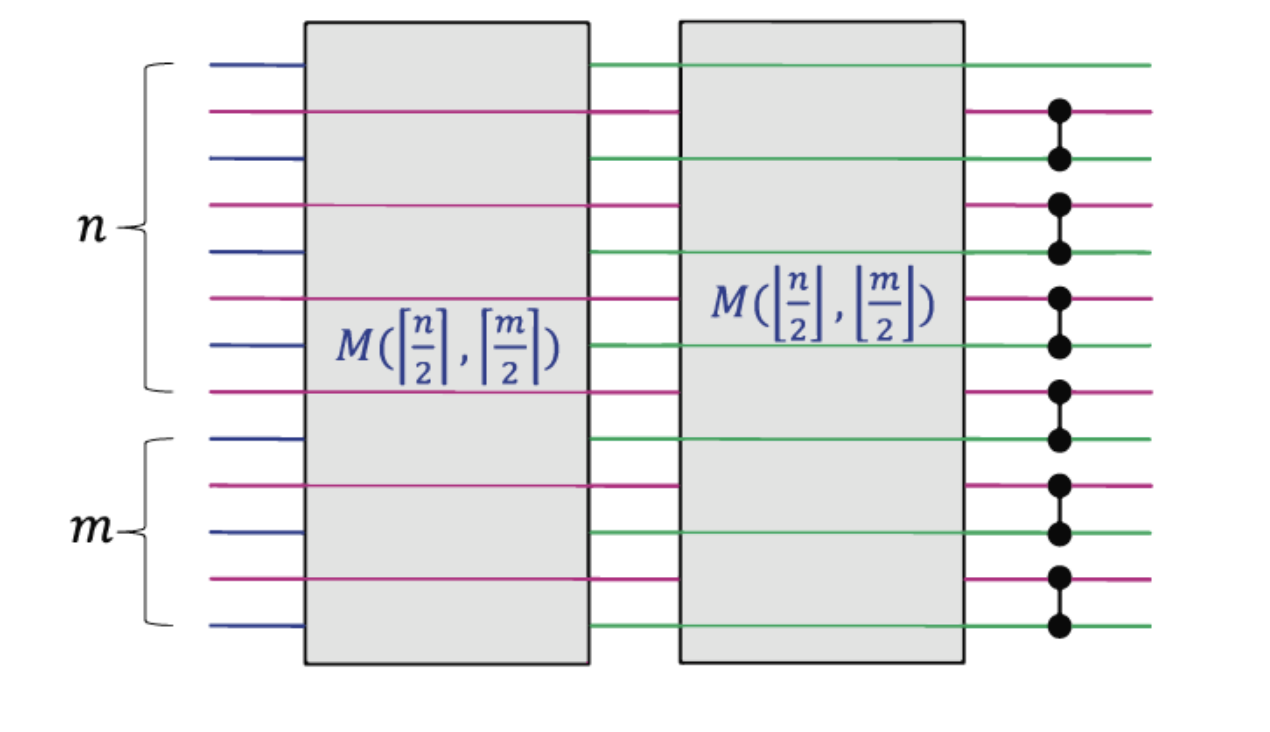
\includegraphics[width=\textwidth]{sorting_network.png}

    \begin{enumerate}
     \item Покажите, что такая сеть действительно сливает два отсортированных массива.
         \item Каково будет общее число компараторов в такой сети?
     \item Какова будет глубина такой сети?
    \end{enumerate}

\end{enumerate}

\subsection{Решения}

\begin{enumerate}

    \item
        Решение с использованием сортировки было бы достаточно простым, но оно не укладывается в ограничение по времени,
        так как требует $\O(n \log n)$ времени.

        В этом случае ответом было бы значение: $\max\left(\max(a_1, l - a_n), \max\left(\frac{a_{i+1} - a_i}{2}\right)\right)$

        \begin{itemize}

            \item
                $\max(a_1, l - a_n)$ учитывает расстояние от крайних точек улицы до ближайших фонарей,

            \item
                $(\frac{a_{i+1} - a_i}{2})$ — половина максимального расстояния между соседними фонарями,
                так как они будут освещать этот промежуток с обеих сторон.

        \end{itemize}

        Для достижения $\O(n)$ разобьём улицу на $n + 1$ равных отрезков и для каждого фонаря определим,
        в каком отрезке он находится $\left\lfloor \frac{a[i]}{l / (n + 1)} \right\rfloor$.

        При таком разбиении гарантируется, что как минимум один из отрезков
        не будет содержать фонарей, поэтому расстояния между фонарями внутри одного отрезка можно не учитывать.

        Для каждого отрезка будем хранить минимальную и максимальную позиции фонарей в нём.
        Чтобы найти минимальное $d$, пройдёмся по непустым отрезкам слева направо и для каждого отрезка
        определим разницу между максимумом левого отрезка и минимумом правого.

        Ответом будет максимум из всех таких разностей пополам.
        Кроме того, не забудем учесть расстояния от крайних точек улицы до ближайших фонарей.

        Сложность такого алгоритма — $\O(n)$, как по времени, так и по памяти.

    \item
        Для решения задачи нужно убедиться, что в массиве длины $n$ присутствуют все числа от $0$ до $n-1$ включительно,
        и найти первое число, которого нет в массиве.

        Алгоритм можно построить следующим образом:

        \begin{itemize}

            \item Пройдемся по каждому элементу массива и попытаемся поставить его в позицию, соответствующую его значению,
            если оно не выходит за границы массива. При этом будем использовать операции обмена элементов (swap),
            чтобы не задействовать дополнительную память. Таким образом, каждый элемент будет "переходить" на своё место.

            \item Если элемент выходит за границы массива, мы оставляем его на текущей позиции и игнорируем.

            \item После завершения перестановки всех элементов, мы еще раз проходим по массиву и находим первый элемент,
            который не совпадает с его позицией. Это и будет минимальное неотрицательное число, отсутствующее в массиве.

        \end{itemize}

        Алгоритм имеет временную сложность $\O(n)$, поскольку каждый элемент перемещается не более одного раза.
        Дополнительная память составляет $\O(1)$, так как мы используем только существующий массив для выполнения перестановок.

    \item \dots

    \item \dots

    \item \dots

    \item \dots

\end{enumerate}
